%-  LaTeX source file

%-  performance.tex ~~
%
%   This is the fourth section of the paper.
%
%                                                   ~~ last updated 24 Sep 2018

\subsection{Profiling of the performance of the end-to-end workflow on Titan}
\label{subsec:profiling}

% For two-column wide figures use
\begin{figure*}
% Use the relevant command to insert your figure file.
% For example, with the graphicx package use
  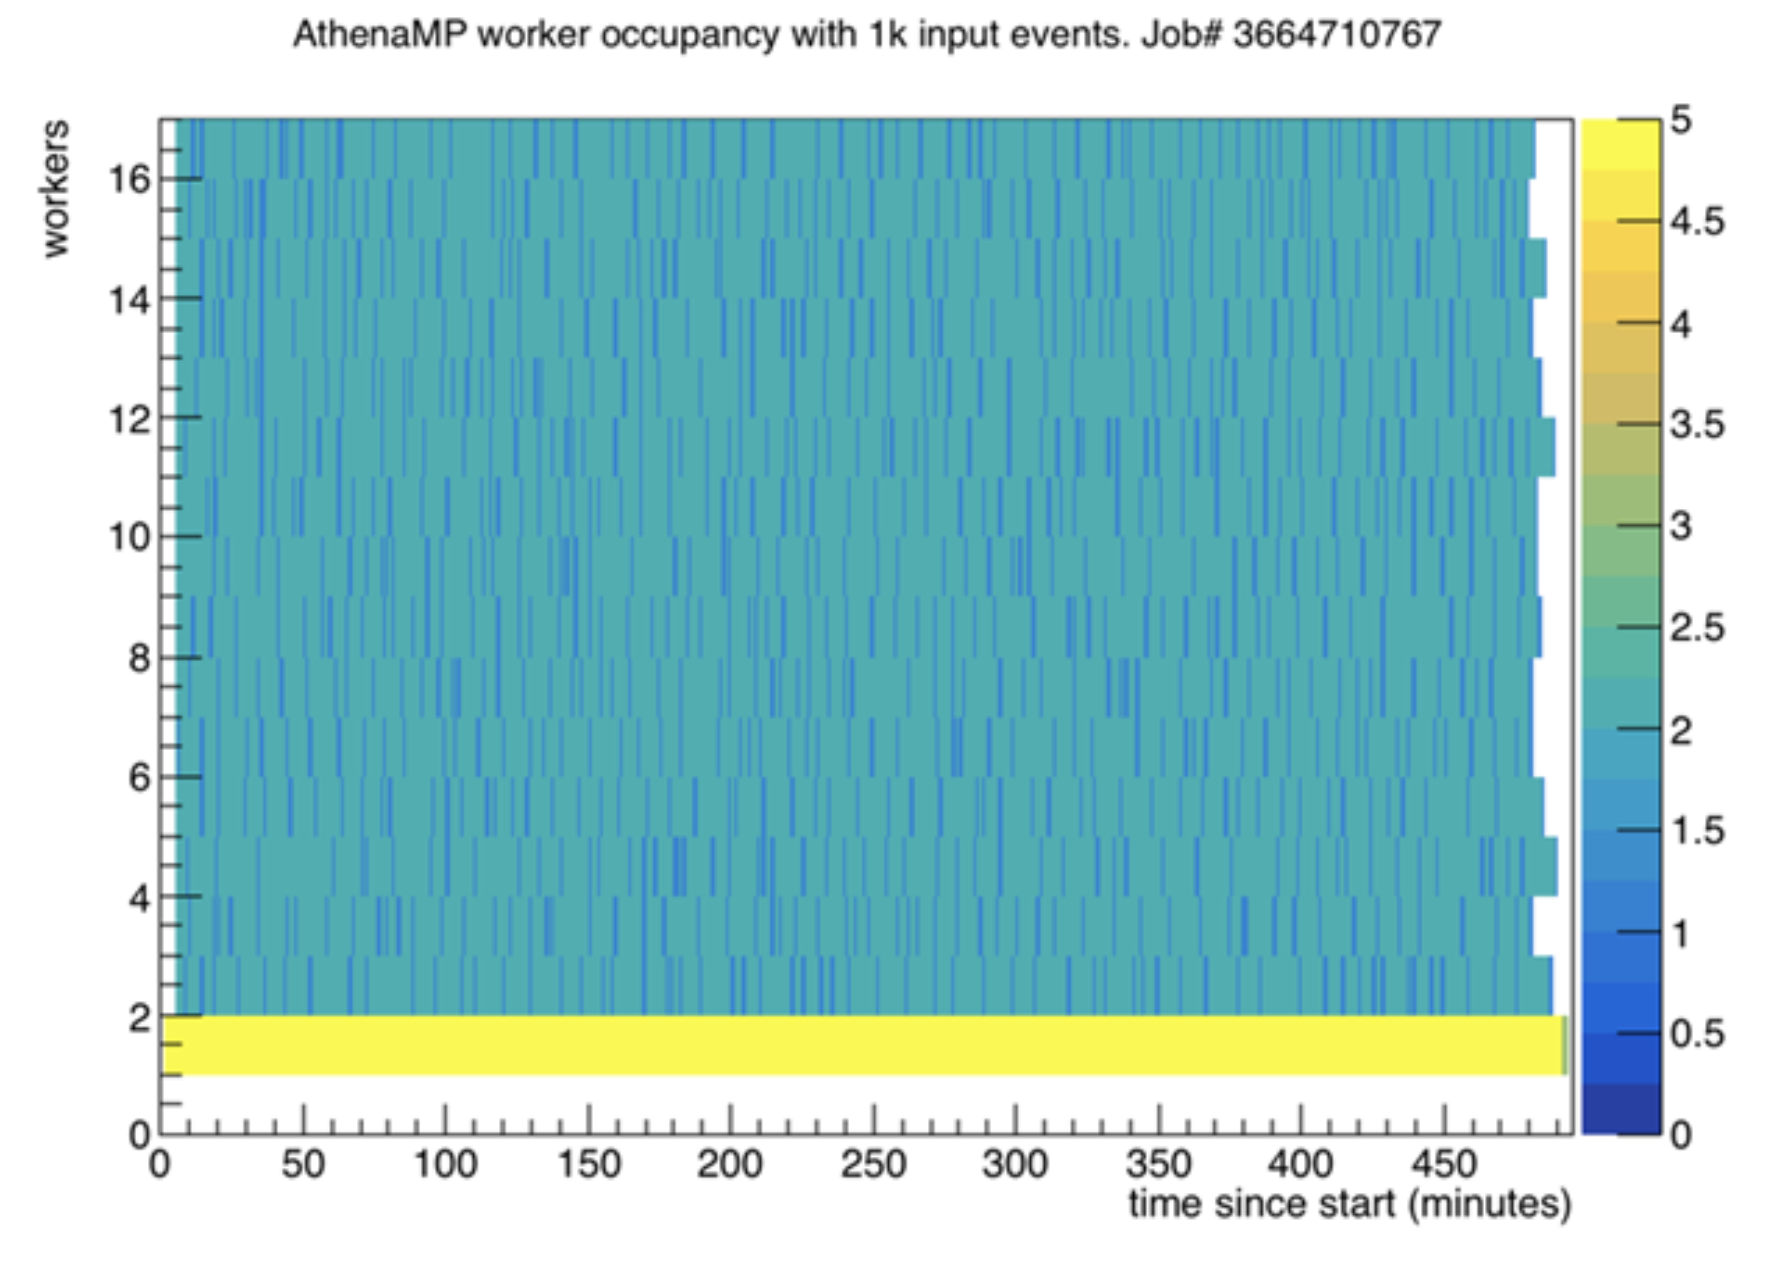
\includegraphics[width=0.75\textwidth]{images/Figure_6_placeholder.png}
% figure caption is below the figure
\caption{AthenaMP worker occupancy for typical ATLAS detector simulation job
with 1000 input events}
\label{fig:athena1000}
\end{figure*}

% For two-column wide figures use
\begin{figure*}
% Use the relevant command to insert your figure file.
% For example, with the graphicx package use
  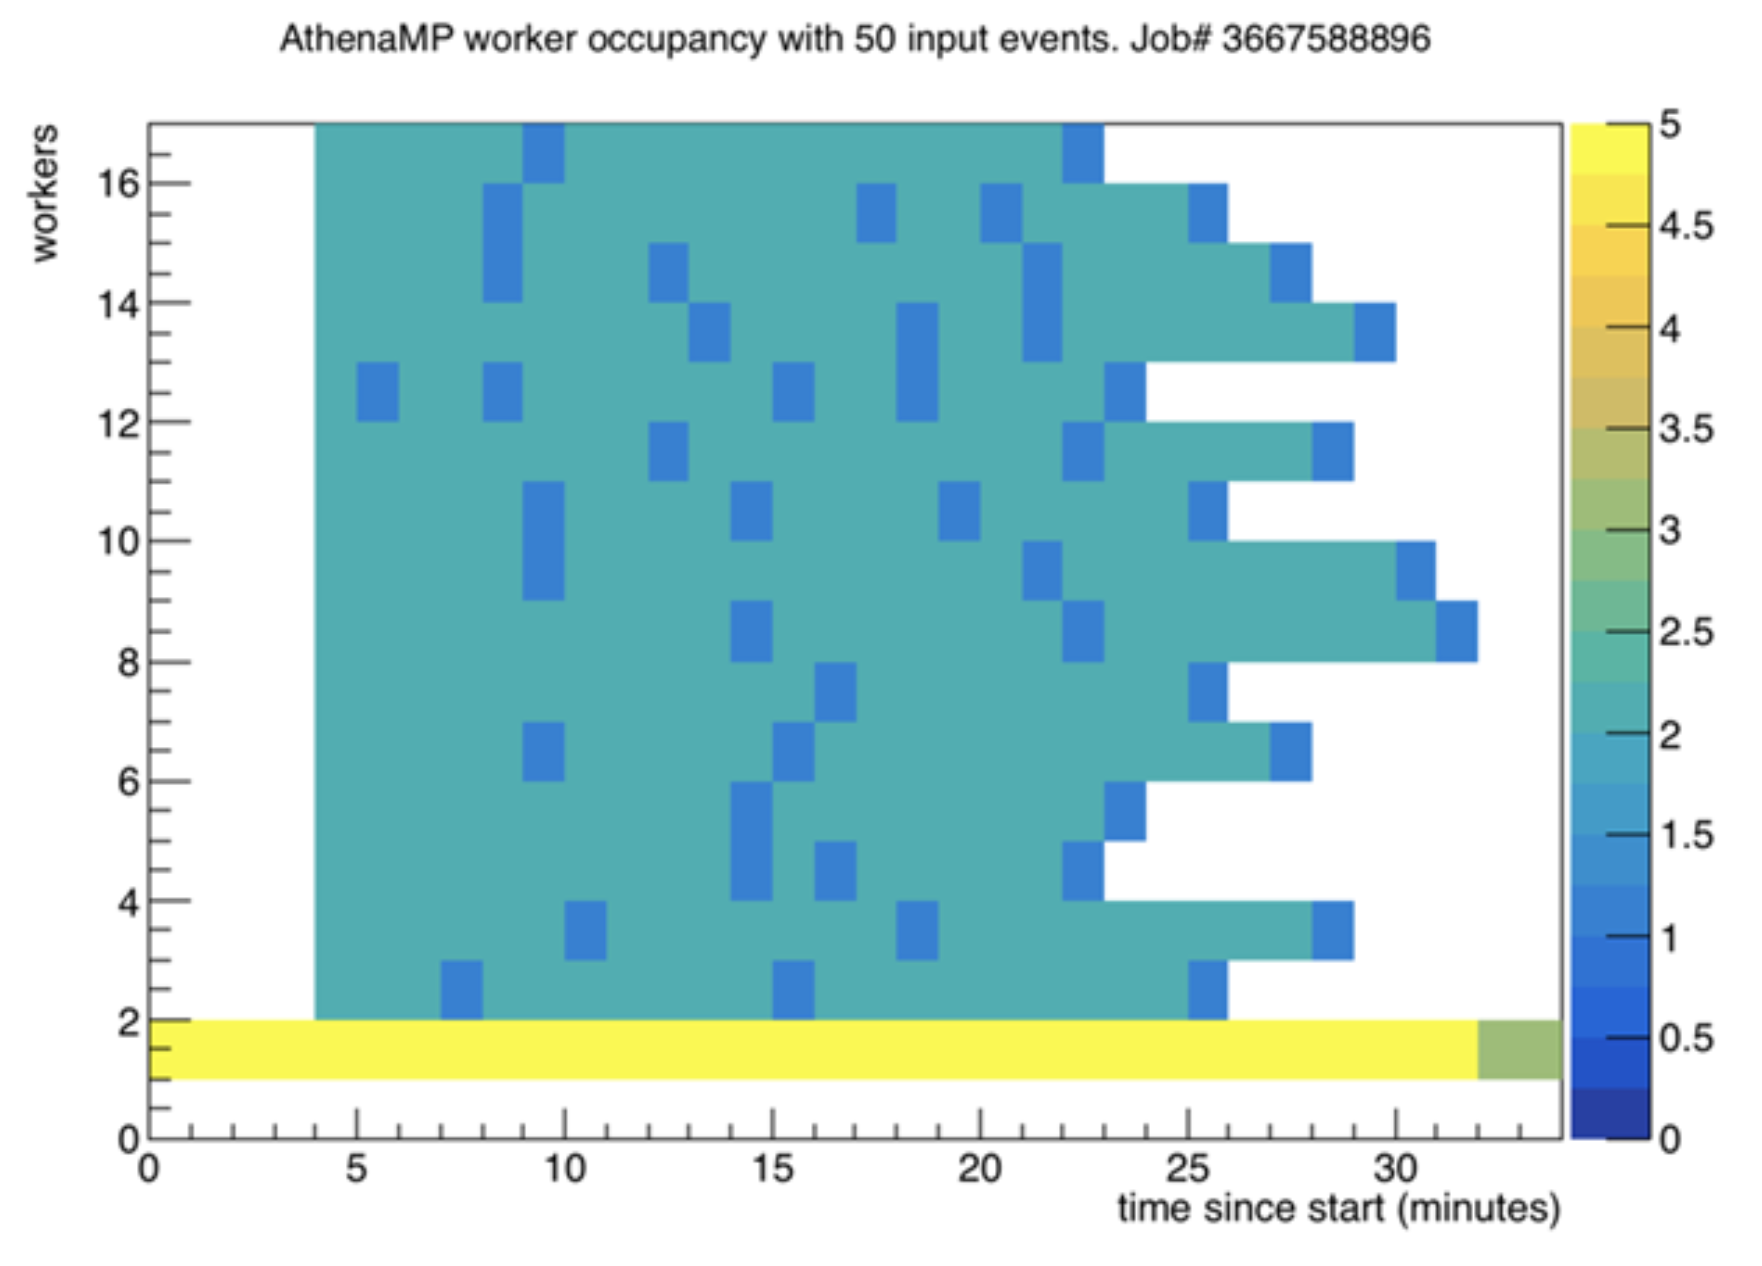
\includegraphics[width=0.75\textwidth]{images/Figure_7_placeholder.png}
% figure caption is below the figure
\caption{AthenaMP worker occupancy for typical ATLAS detector simulation job
with 50 input events.}
\label{fig:athena50}
\end{figure*}

\begin{itemize}
    \item There are two primary objectives:
    \item %
        \begin{enumerate}
            \item some way to characterize the performance (efficiency) of
                PanDa to perform WLMS on LCF (internal), and
            \item some way to characterize the impact of PanDA on Titan
                (external facing).
        \end{enumerate}
    \item Abstract Model of Workload Management System: The common
        functionality that ``all'' distributed workload management systems
        perform, include:
        \begin{itemize}
            \item Manage Payload (i.e., the full set of application workflow)
            \item Get resource information
            \item T2 function of N
            \item Workload Shaping: i.e., decompose Payload into tasks
            \item Job Shaping: i.e., bundle tasks into jobs of defined
                configuration on a resource
            \item Execution management i.e., submit/launch jobs and ensure
                completeness
            \item Data and metadata management, i.e., update central POP with
                job state information.
        \end{itemize}
\end{itemize}

Trying to derive the TTC using the above abstract model of D-WLMS should be our
goal, not a fine grain description of time taken.

These are categories of functionality, not necessarily states. Not all
categories will be exclusive (i.e., unlike states of a job). 

Suggest as a possible consideration to consider the production stream

\subsection{Impact of ATLAS CSC108 on Titan}
\label{subsec:csc108}

The CSC108 project operates under the assumption that the constraints imposed
on its jobs by OLCF prevent it from competing for resources with other
projects. In order to assess the effectiveness of this strategy, we have
pursued several lines of inquiry by sampling data from the MOAB scheduler on
Titan.

Note that code supporting this section is available at
\url{https://github.com/ATLAS-Titan/moab-data}. 

\subsubsection{Blocking Probability}
\label{subsubsec:blockingprobability}

We begin with a simple model that defines an event called a ``block'' and then
detects its occurrences within the data.

Let $C_i$ be the abstract resources in use by CSC108 at the $i^{\text{th}}$
sample point in time, and let $U_i$ be the unused (idle) resources remaining on
Titan. We then define a boolean $B_i$ representing a ``block'' to be 1 if there
exists at least one job at the $i^{\text{th}}$ sample point which requests
$(C_i + U_i)$ resources or less, and we define $B_i$ to be zero otherwise.

Summing $B_i$ over all $i$ gives a count of sample points at which a block
occurred, and dividing that count by the number of total sample points yields a
quantity we will term a ``blocking fraction''.

To use this model for our concrete data set, we define the resources in
question to be requested processors (or requested nodes).

(Specific numbers and graphs go here.)

%-  vim:set syntax=tex:
